The kitting system presented in this document relies on a \textit{direct} model of execution where the executor directly performs the activities specified in the plan. Figure~\ref{fig:executor} depicts the executor process for the kitting domain where ellipses represent files, regular rectangles are used to define processes, and rounded rectangles illustrate tools. The red dashed box contains the processes part of the executor. The components in Figure~\ref{fig:executor} are described below:
\begin{itemize}
\item[$1.$] PDDL domain and problem files are used by a planner to generate a plan file. The plan file contains a sequence of actions that can be executed from the initial state and that leads to a goal state. The actions present in the plan file are originally defined in the PDDL domain file. The initial and goal states are defined in the PDDL problem file.
\item[$2.$] The interpreter takes the plan file as input and builds the corresponding CRCL file. The knowledge representation is required to locate objects in the environment. Table~\ref{tab:takepart} shows an example of CRCL commands generated for the PDDL action \stvar{take-part(part\_b\_1)}. Please note that the PDDL action \stvar{take-part} developed for the current kitting domain has more than one parameter. All the parameters are not relevant for the example depicted in Table~\ref{tab:takepart} and the number of parameters has been subsequently reduced for simplicity.

\begin{table}[h!]
\centering

    \begin{tabular}{l}
    \stvar{take-part(part\_b\_1)}\\
    \hline
    \hline
  \texttt{\scriptsize{Message (``take part part\_b\_1")}}\\
  \texttt{\scriptsize{MoveTo(\{\{-0.03, 1.62, -0.25\}, \{0, 0, 1\}, \{1, 0, 0\}\})}}\\
  \texttt{\scriptsize{Dwell (0.05)}}\\
  \texttt{\scriptsize{MoveTo(\{\{-0.03, 1.62, 0.1325\}, \{0, 0, 1\}, \{1, 0, 0\}\})}} \\
  \texttt{\scriptsize{CloseGripper ()}} \\
  \texttt{\scriptsize{MoveTo(\{\{-0.03, 1.62, -0.25\}, \{0, 0, 1\}, \{1, 0, 0\}\})}}\\
  \texttt{\scriptsize{Dwell (0.05)}}\\
  \hline
  \end{tabular}
\caption{An example of CRCL commands for a PDDL action.}
  \label{tab:takepart}
\end{table}
\item[$3.$] The CRCL file is used by the controller in order to create ROS commands.
\item[$4.$] The ROS commands are used by the ROS software controller for a robotic arm to initiate actual execution of actions.

\end{itemize}

%The \textit{indirect} model tracks the execution of the plan while human agents perform the plan activities. Both models of execution require tools to monitor failures that are likely to emerge during a plan execution.


%
%\begin{figure}[h!]
%\centering
%\scalebox{.7}{
%\begin{tikzpicture}[node distance=1.5cm, every edge/.style={link}]
%
%  %%-- Domain file
%  \node[attribute] (domain) {PDDL Domain};
%  %%-- Empty node to center the planner node that comes right below it
%  \node[empty] (empty) [right=0.5cm of domain]{};
%  %%-- Problem file
%  \node[attribute] (problem) [right=0.5cm of empty] {PDDL Problem};
%  %%-- Planner
%  \node[entity] (planner) [below=1cm of empty] {$1.$ Planner};
%  %%-- Plan
%  \node[attribute] (plan) [below=0.5cm of planner] {Plan};
%  %%-- Knowledge Representation
%  \node[output] (database) [left=1cm of plan] {Knowledge Representation};
%  %%-- Interpreter
%  \node[entity] (interpreter) [below=1cm of plan] {$2.$ Interpreter};
%  %%-- CRCL
%  \node[attribute] (crcl) [below=0.5cm of interpreter] {CRCL};
%  %%-- Controller
%  \node[entity] (controller) [below=0.5cm of crcl] {$3.$ Controller};
%  %%-- ROS commands
%  \node[entity] (ros) [below=1cm of controller] {$4.$ ROS};
%  %%-- Robotic Arm
%%  \node[output] (arm) [below=1cm of ros] {Robotic Arm};
%
%  \draw[myarrow] (domain.south) -- ++ (0,-1)  |-  (planner.west);
%  \draw[myarrow] (problem.south) -- ++ (0,-1)  |-  (planner.east);
%  \draw[myarrow] (planner.south) -- (plan.north);
%  \draw[myarrow] (plan.south) -- (interpreter.north);
%  \draw[myarrow] (interpreter.south) -- (crcl.north);
%  \draw[myarrow] (crcl.south) -- (controller.north);
%  \draw[myarrow] (controller.south) -- (ros.north);
%  %\draw[myarrow] (ros.south) -- (arm.north);
%  %\draw[thick,decorate,decoration={brace,amplitude=10pt,mirror,raise=4pt},yshift=0pt]
%  %     (4.5,-10) -- (4.5,-4.2) node[midway, right=15pt]{Executor};
%  \draw[myarrow] (database.south) -- ++ (0,-1)  |-  (interpreter.west);
%
%  %\draw[red,thick,dotted] ($(interpreter.north west)+(-0.5,0.6)$)  rectangle ($(controller.south east)+(0.5,-0.6)$) node [rotate=90, right=of interpreter] {Executor};
%  \draw[red,thick,dotted] ($(interpreter.north west)+(-0.5,0.6)$)  rectangle ($(controller.south east)+(0.5,-0.6)$);
%
%\end{tikzpicture}
%}
%\caption{The executor process.}
%\label{fig:executor}
%\end{figure}



\begin{figure}[ht]
\begin{center}
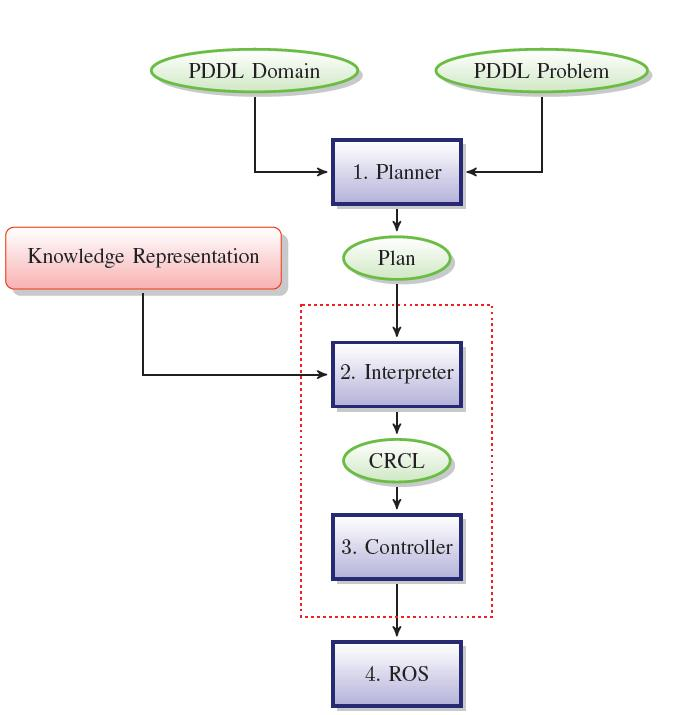
\includegraphics[width=8cm]{images/executordiag.jpg}
\caption{The executor process.}
\label{fig:executor}
\end{center}
\end{figure}

During execution, kitting fails to reach its full potential for savings when the supply chain fails and parts and components are not available for kit construction, or when a kit is not properly filled. Part availability failures can be triggered by inaccurate information on the location of the part or part shortage due to delays in internal logistics. Kit construction errors may be due to problems such as improper equipment setup, improper equipment maintenance, part damage, wrong type of part, or part dropped by the robot.


Models for detecting and recovering from plan execution failures mostly deal with \textit{precondition failures}, \textit{action failures}, and \textit{unattributable failures}~\cite{Myers1998}. Precondition failures appear when all the preconditions for a PDDL action are not met during the execution of this action. Action failures are encountered when the execution of an action does not attain its intended effects. Unattributable failures occur when unexpected events caused by external agents change a random part of the environment, thus causing the current plan to become obsolete.

Some metrics revolving around the three aforementioned failure concepts are listed below:
\begin{itemize}
\item \sf Manipulation robustness \rm -- Qualitative functionality metrics that describe how well a robot can handle complex objects in complex environments without failing or requiring additional operator interventions. Failures can occur during object detection (lightning variation, shadows), object approach (partially buried), and object manipulation (fragile) operations.\\
\item \sf Transporting components \rm -- Qualitative metrics that describe how well a robotic arm can grasp objects and move these objects from an initial position to a goal position without dropping them.\\
\item \sf Plan generation \rm -- As mentioned previously, failures are susceptible to happen in kitting during the execution of CRCL commands, causing the current plan to become obsolete. In some cases, the current state of the environment is brought back to the state prior to the failure and the robot starts from a ``stable" state. In other cases a completely new plan is generated by the planning system where the robot starts all over. Previous experience suggests that the latter solution is preferable considering it will take less time to generate a new plan than going back to a previous state from the original plan.

    However, the state of the environment after a failure may be closer to the goal configuration and a complete replanning may take longer. In this case, the most time effective action sequence that leads to the goal state is used by the system.\\
\item \sf Contact errors \rm -- Quantitative metrics that keep track of the number of collisions between the robotic arm and objects in the environment. The performance of the robotic arm during kit building is affected by the position of joints and end-effector in the environment. The position of the end-effector can reduce the time to complete tasks but can also increase the number of collisions due to joint contact with other objects in a confined space.\\
%\item \sf Action effects \rm -- Table~\ref{tab:takepart} represents the PDDL action . \\
\item \sf Failures during kit building\rm -- Quantitative metrics the report the total number of failures encountered during kit building. When a failure arises during the building of a kit, the system may generate a new plan to recover from the failure. If a failure occurs during the execution of the new plan, different or not from the previous one, the number of failures for building the current kit is incremented and this number is now 2. The number of failures for building a kit is not related to the plan itself but with the construction of the finished kit. \\
\item \sf Failure modes recovery \rm -- Quantitative metrics that represent the number of failure modes the system recovers from through the use of contingency plans. When a failure is detected in the execution process, failure monitors encode appropriate responses (contingency plans) to failure modes for this particular failure.\\

\end{itemize}
